\documentclass{article}
\usepackage{titling}
\usepackage{scrextend}
\usepackage{xcolor}
\usepackage{graphicx}
\usepackage{tipa}
\usepackage{hyperref}
\usepackage{lipsum}
\usepackage{blindtext}
\usepackage{multicol}
\usepackage[export]{adjustbox}
\usepackage{newspaper}
\usepackage[margin=1in,tmargin=0.75in]{geometry}

\newcommand{\PutTitle}[1]
{
    \begin{center}
        {\huge\bfseries\thetitle}\\
        by \theauthor\\
        \thedate\\
        #1        
    \end{center}
    \hrule
    \vspace{2ex}
}

\setlength\paperwidth{8.5in}
\setlength\paperheight{11in}
\setlength\parindent{24pt}

\hypersetup
{
    colorlinks=true,
    linkcolor=blue,
    urlcolor=blue,
}

\title{BINGO Project \#3}
\author{Jonah Mondragon}
\date{\today}

\begin{document}

\PutTitle{English Period 8}
\pagestyle{headings}
\thispagestyle{empty}

\section{Academic Vocabulary Book}
Create a dictionary with the following Academic Vocabulary:
\begin{addmargin}[0.5in]{0in}
    \subsection*{Alliteration}
        A form of rhyme that involves the start of words rather then the end.
    \subsection*{Allusion}
        A subtly implied reference to something external to the context of the implication; often with the purpose of comedic
        effect.
    \subsection*{Characterization}
        The profile of a character; the analysis, or observation, of someone's tendencies or disposition.
    \subsection*{Foreshadowing}
        A reference made within a fictional context referring to a future event; typically a near disaster, or the ending. 
    \subsection*{Homonym}
        Two words with the same sound---with the possibility of sharing the same spelling as well---but with difference in
        meaning.
    \subsection*{Imagery} 
        Language delivered with the purpose of conveying a scene (or an image) to the reader/observer.
    \subsection*{Irony}
        A situation in which an entity's expected behavior is either the exact opposite of reality, or intensely the same.
    \subsection*{Metaphor}
        A methodology used in an either literary or conversational sense to convey a new concept to another person; using 
        their prior knowledge of some other concept; or something simple enough that the connection can be either humorous
        and/or enlightening.
    \subsection*{Monologue}
        An intentional form of rambling; typically put into action when encountered by an immensely dense subject;
        particularly a self-indulged subject.
    \subsection*{Oxymoron}
        A situation where two antonyms are used together to form a practical idea; ``deadly alive''; ``drowned vividness.''
    \subsection*{Persona}
        Only one simple aspect of someone's personality; perhaps as a public figure; or an entity with mannerisms.
    \subsection*{Personification}
        The application of a personality to an otherwise inanimate object; or a more instinctual entity.
    \subsection*{Prologue}
        An introduction; the exact implementation is defined by the application.
    \subsection*{Pun}
        A play on words.
    \subsection*{Rising Action}
        An event, or set of events, that ultimately lead to the climax or the need for the climax.
    \subsection*{Soliloquy}
        The notion whereby one's inner thoughts can converse themselves aloud unconsciously; whether when alone or 
        accompanied by other people. Usually used within observed fictional stories with the intention of allowing the
        audience to understand the concerns/motives of the character.
    \subsection*{Sonnet}
        A poem whose verses contain 14 lines and are generally written via means of iambic pentameter (iambic pentameter
        meaning; 10 syllables on a single line; and one of every two are stressed; a phenomenon that often occurs 
        naturally in the use of English).
    \subsection*{Synonym}
        A word with a similar or interchangeable definition with another; country and county.
    \subsection*{Tableau}
        Imagery with very precise accuracy.
    \subsection*{{\color{red}The{\color{blue}me}}}
        One central idea that many objects involved refer to; in storytelling, it can be thought of as
        ``{\color{red}the}\textpipe{\color{blue}me}ssage.''
\end{addmargin}

\section{Acrostic Poem}
\begin{addmargin}[0.8in]{0.8in}
    Maybe I was too giddy, \\
    Awkward, perhaps; but no; she told me explicitly otherwise. \\
    Reaching around her shoulder; heartrate playing the gypsy; \\
    Inclined to the possibility of stealing a kiss. \\
    Allow my head to tilt toward; or climb inward into a frenzy? \\
    Humbling, hopefully, with the words ``next time''; thus instilling forward bliss. \\
\end{addmargin}

\section{Newspaper}
\vspace{0.5in}
{
\date{February 19, 1598}
\SetPaperName{Verona Times}
\SetPaperPrice{TWO DOLLARS}
\SetPaperSlogan{``I don't remember the books I have read any more then the meals I have eaten; even so, they have made me''}
\SetPaperLocation{Verona, Italy}
\currentvolume{47}
\currentissue{1}
\maketitle

\setlength{\columnsep}{15pt}
\begin{multicols}{3}
    \headline{\sf{The feud of The Montague's and The Capulet's}}
    The only conflict which has plagued our fair city for centuries has been between the Montague's and the Capulet's; two well esteems lineages, with vast influences upon Verona. 
    Chief among these are the Capulet's ownership of Piazza Delle Erbe marketplace; making for an amiable nest egg. 
    On the side of Mantague's, they only happen to own the Communal Palace, enough said.
    A recent development has put this age-long feud into a bit of a frenzy.
    Tybalt of the Capulet family, a man whom we haven't much information;\footnote{
        In our attempts to facilitate questions of his stature within the Capulet family, Tybalt managed to evade our every request in a rather amazing fashion; involving showing off several disguises of great dexterity and fashionable uses of his sword.}
        was recently killed by Romeo of the Mantague family, surely extenuating the tension of the two families.
    To an utter astonishment, the punishment of this crime was not administered to be death, as is usual for the pretense of murder, but rather banishment;
        this was due to the direct manipulation of the Prince, at who's words resulted in the immediate departure of Romeo, he hasn't been seen since.
    This occurrence can only lead to more brutality on both sides of the spectrum; there's speculation that this wasn't an unprovoked attack, that Tybalt had insinuated the situation; of course speculation also lies in the other direction as well.
    Here at \textit{Verona Times}, we can only hope that future events, such as the Spectacled Burning just a decade ago, doesn't recur as a result of this feud; that it stays within private property, and no innocents are killed.
    \closearticle

    \headline{\bf Revolutionary Dress Apparel}
    Our local clothing store ``Witherfords and Family'' have just created a magnificent new set of apparel, for the (comparatively, within the realm of dress apparel) low, low price of 55 Dollars!
    \begin{center}
    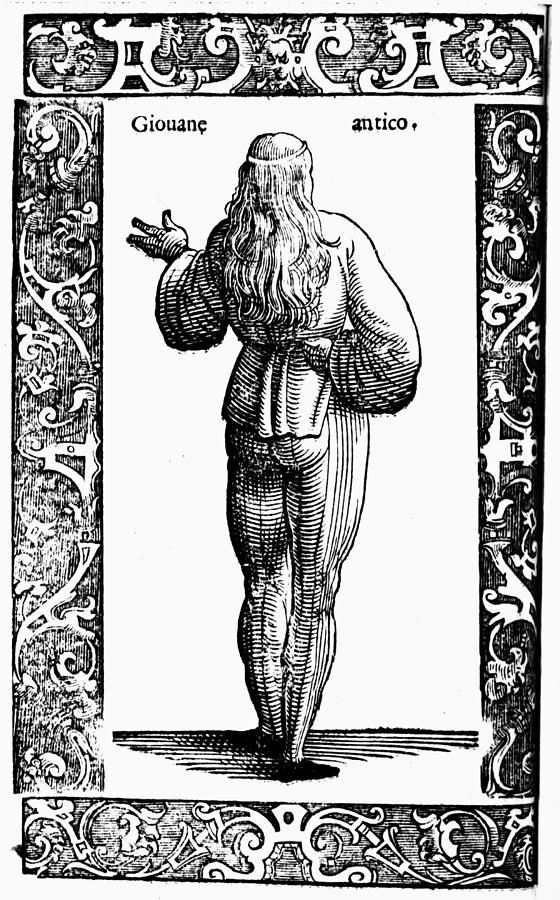
\includegraphics{1598 Fashion.jpeg}
    \end{center}
    \closearticle
    
    \headline{\bfseries Omitted for Brevity...}
    \closearticle
    
    \headline{\ttfamily{Editorial}}
    Long time consumers of the \textit{Verona Times} will know that an editorial section is rarely a concern during it's publication, however it must be emphasized that Romeo is very likely innocent.
    Countless reliable sources tell us so, and the exemption on behalf of the Prince tells significantly of the pretense of this situation; if you happen to see him, on my regard, support him.
    Tybalt was a rather rotten man and not many are supposed to miss him.
    \closearticle
\end{multicols}
}

\section{Artifact Collection}
These are eight artifacts that I believe to be essential to the plot of Romeo and Juliet; along with an explanation of each.
\begin{enumerate}
    \item{Letter:}
        \begin{center}
            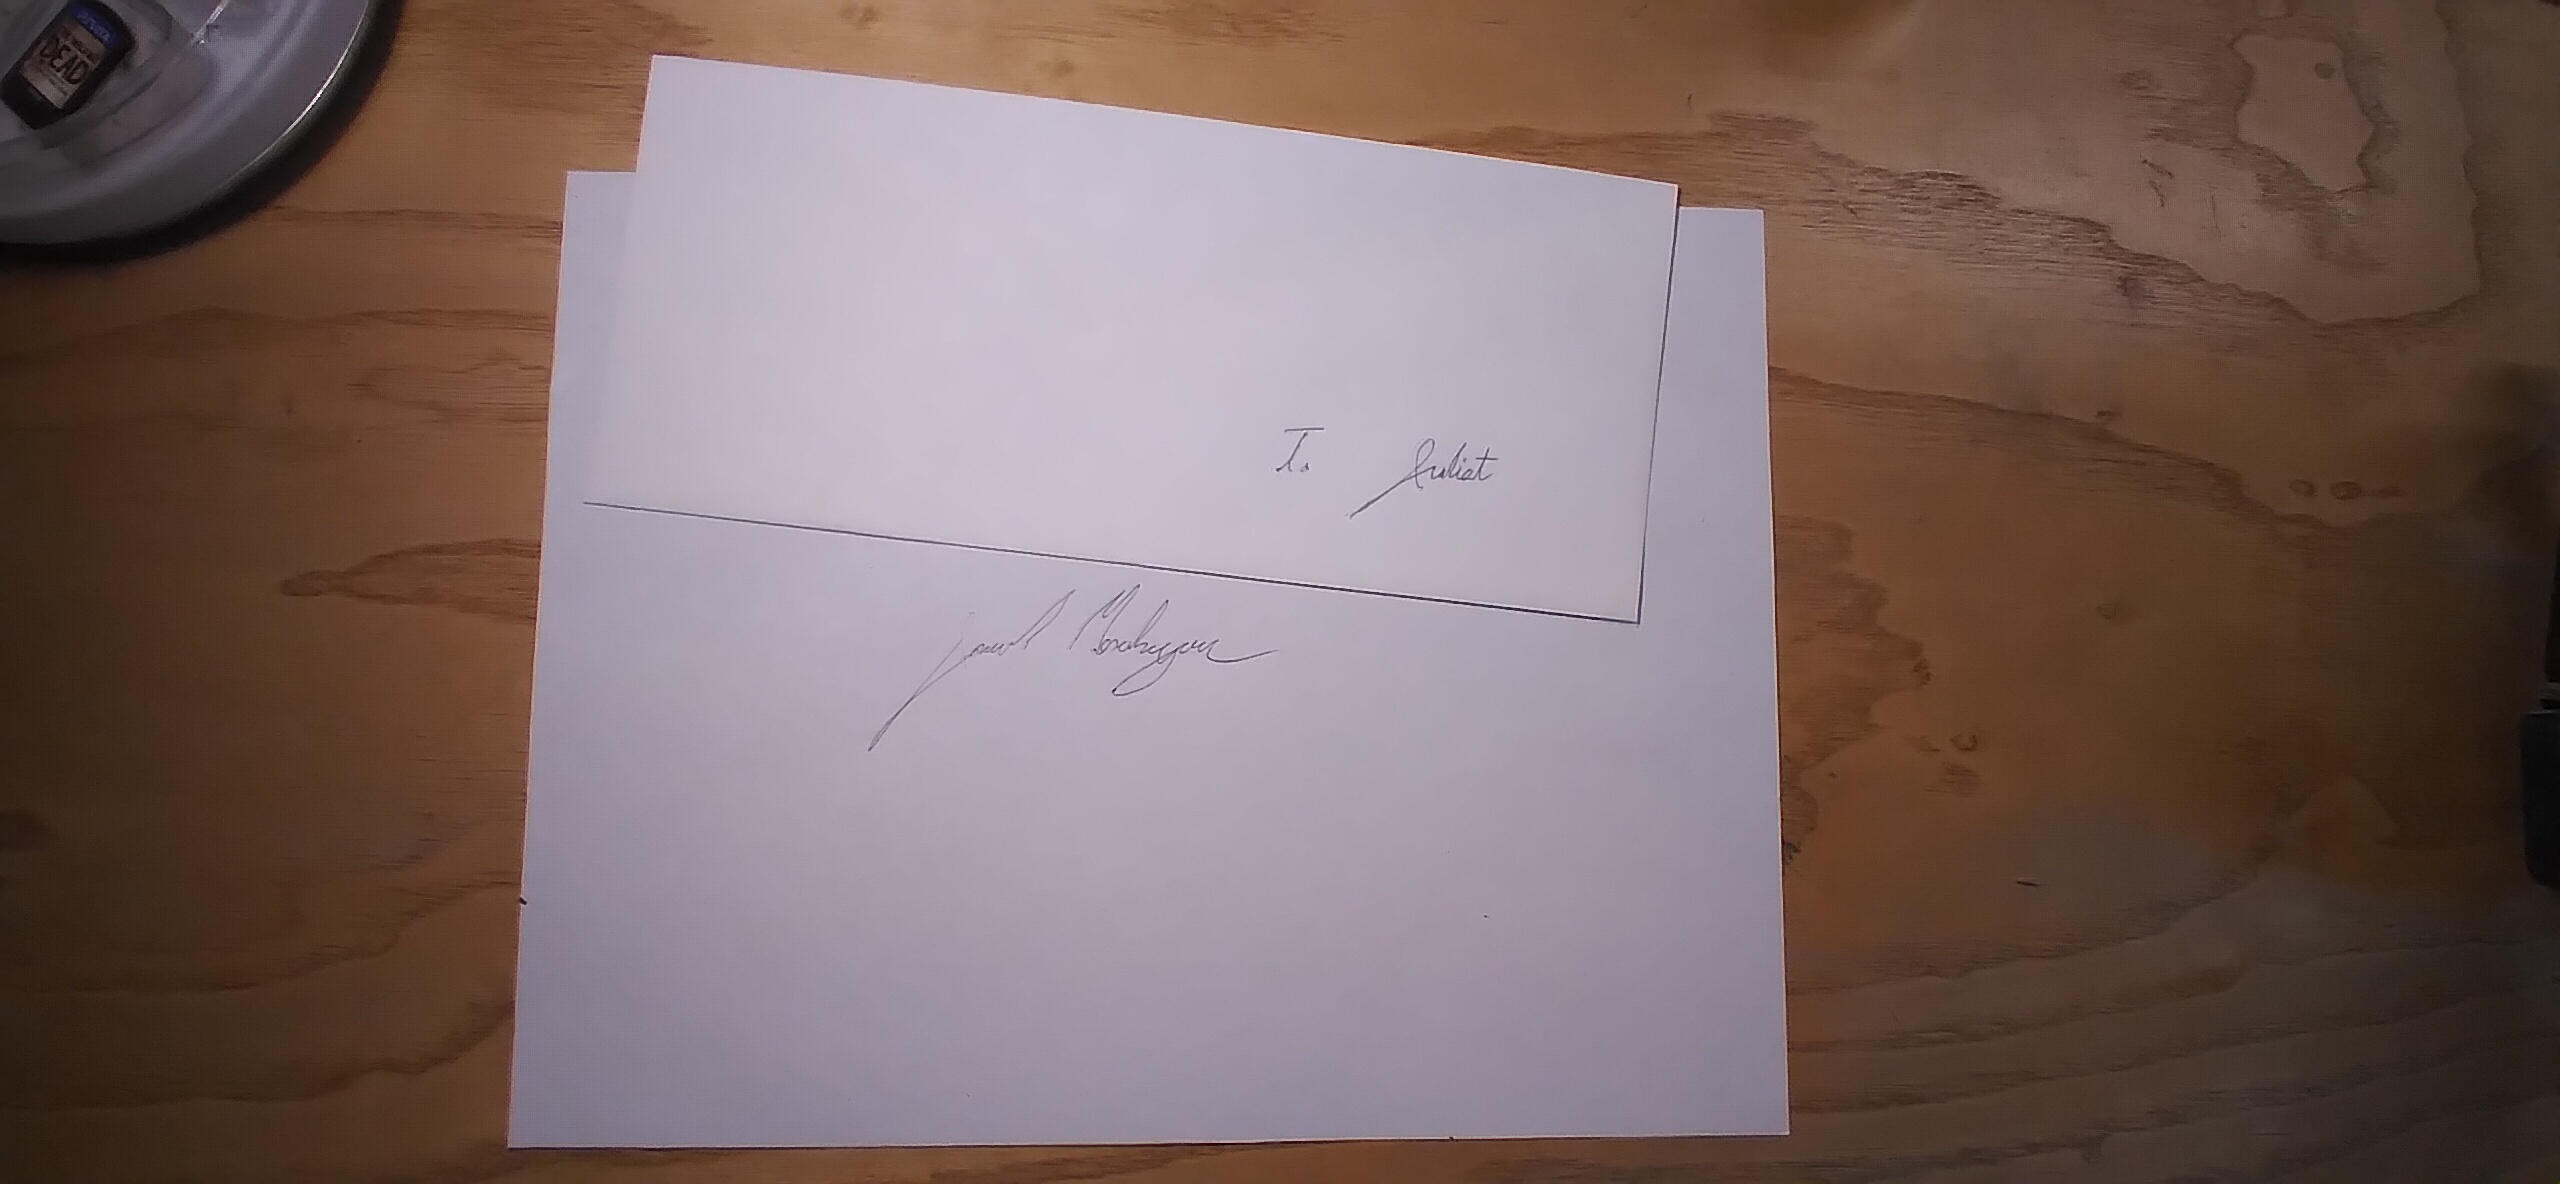
\includegraphics[max width=\textwidth - 6ex]{pics/letter_to_juliet.jpg}
        \end{center}
        \paragraph~
        \lipsum[1]
    \item{Sword:}
        \begin{center}
            %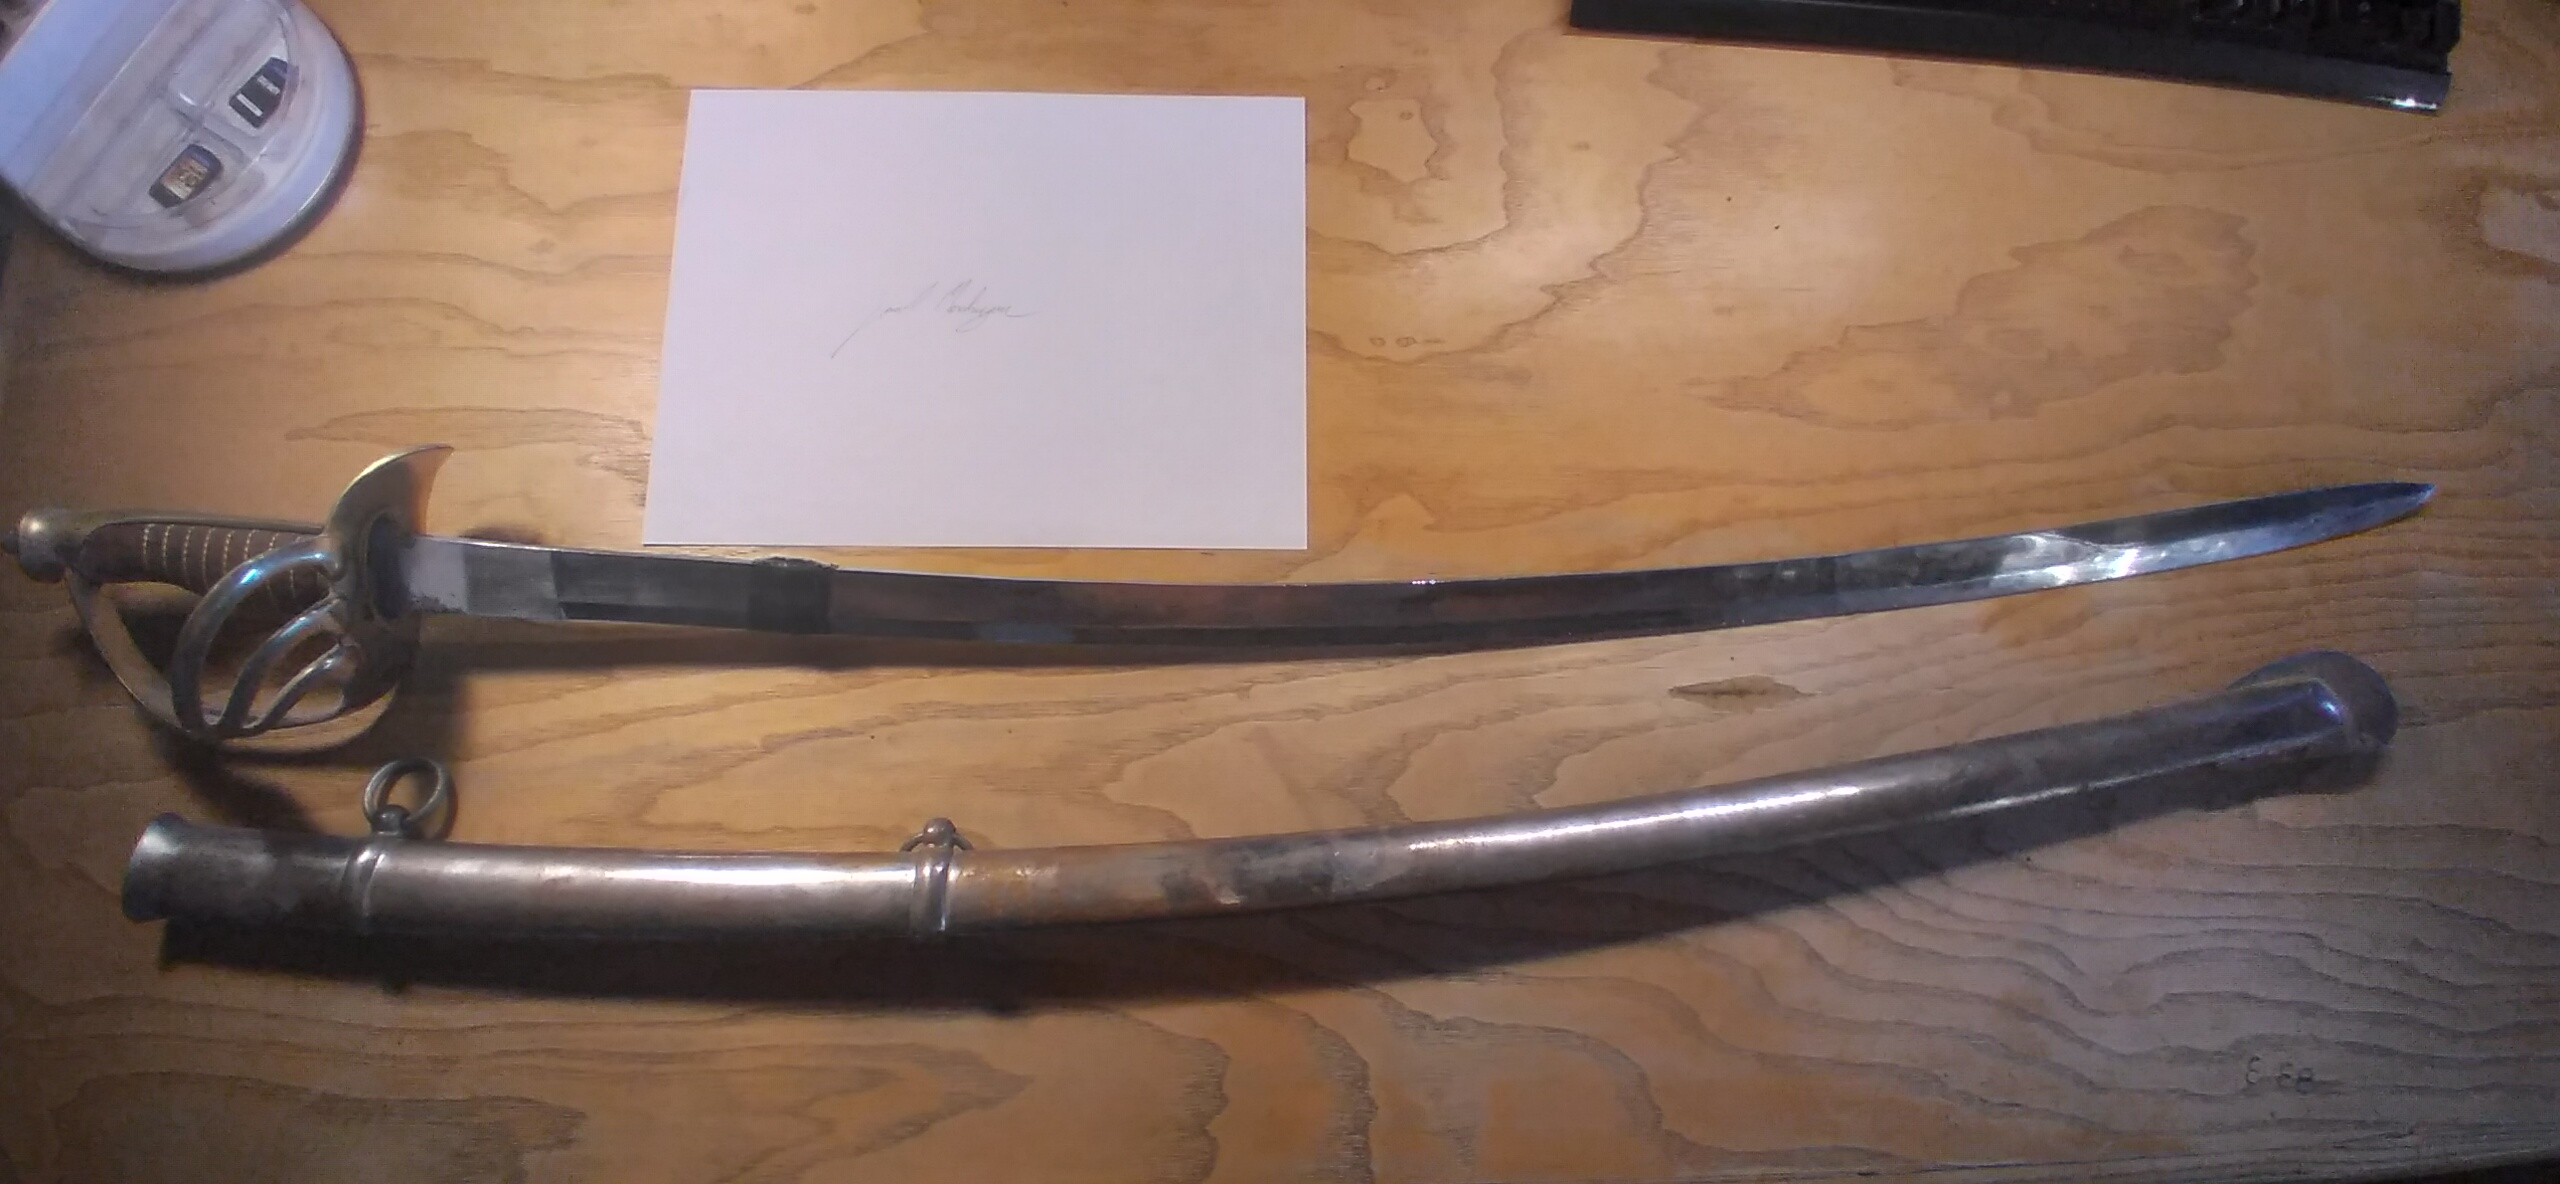
\includegraphics[max width=\textwidth - 6ex]{pics/sword.jpg}
            \includegraphics[max width=\textwidth - 6ex]{pics/necklace.jpg}
        \end{center}
        \paragraph~
        \lipsum[1]
    \item{Rope Ladder:}
        \begin{center}
            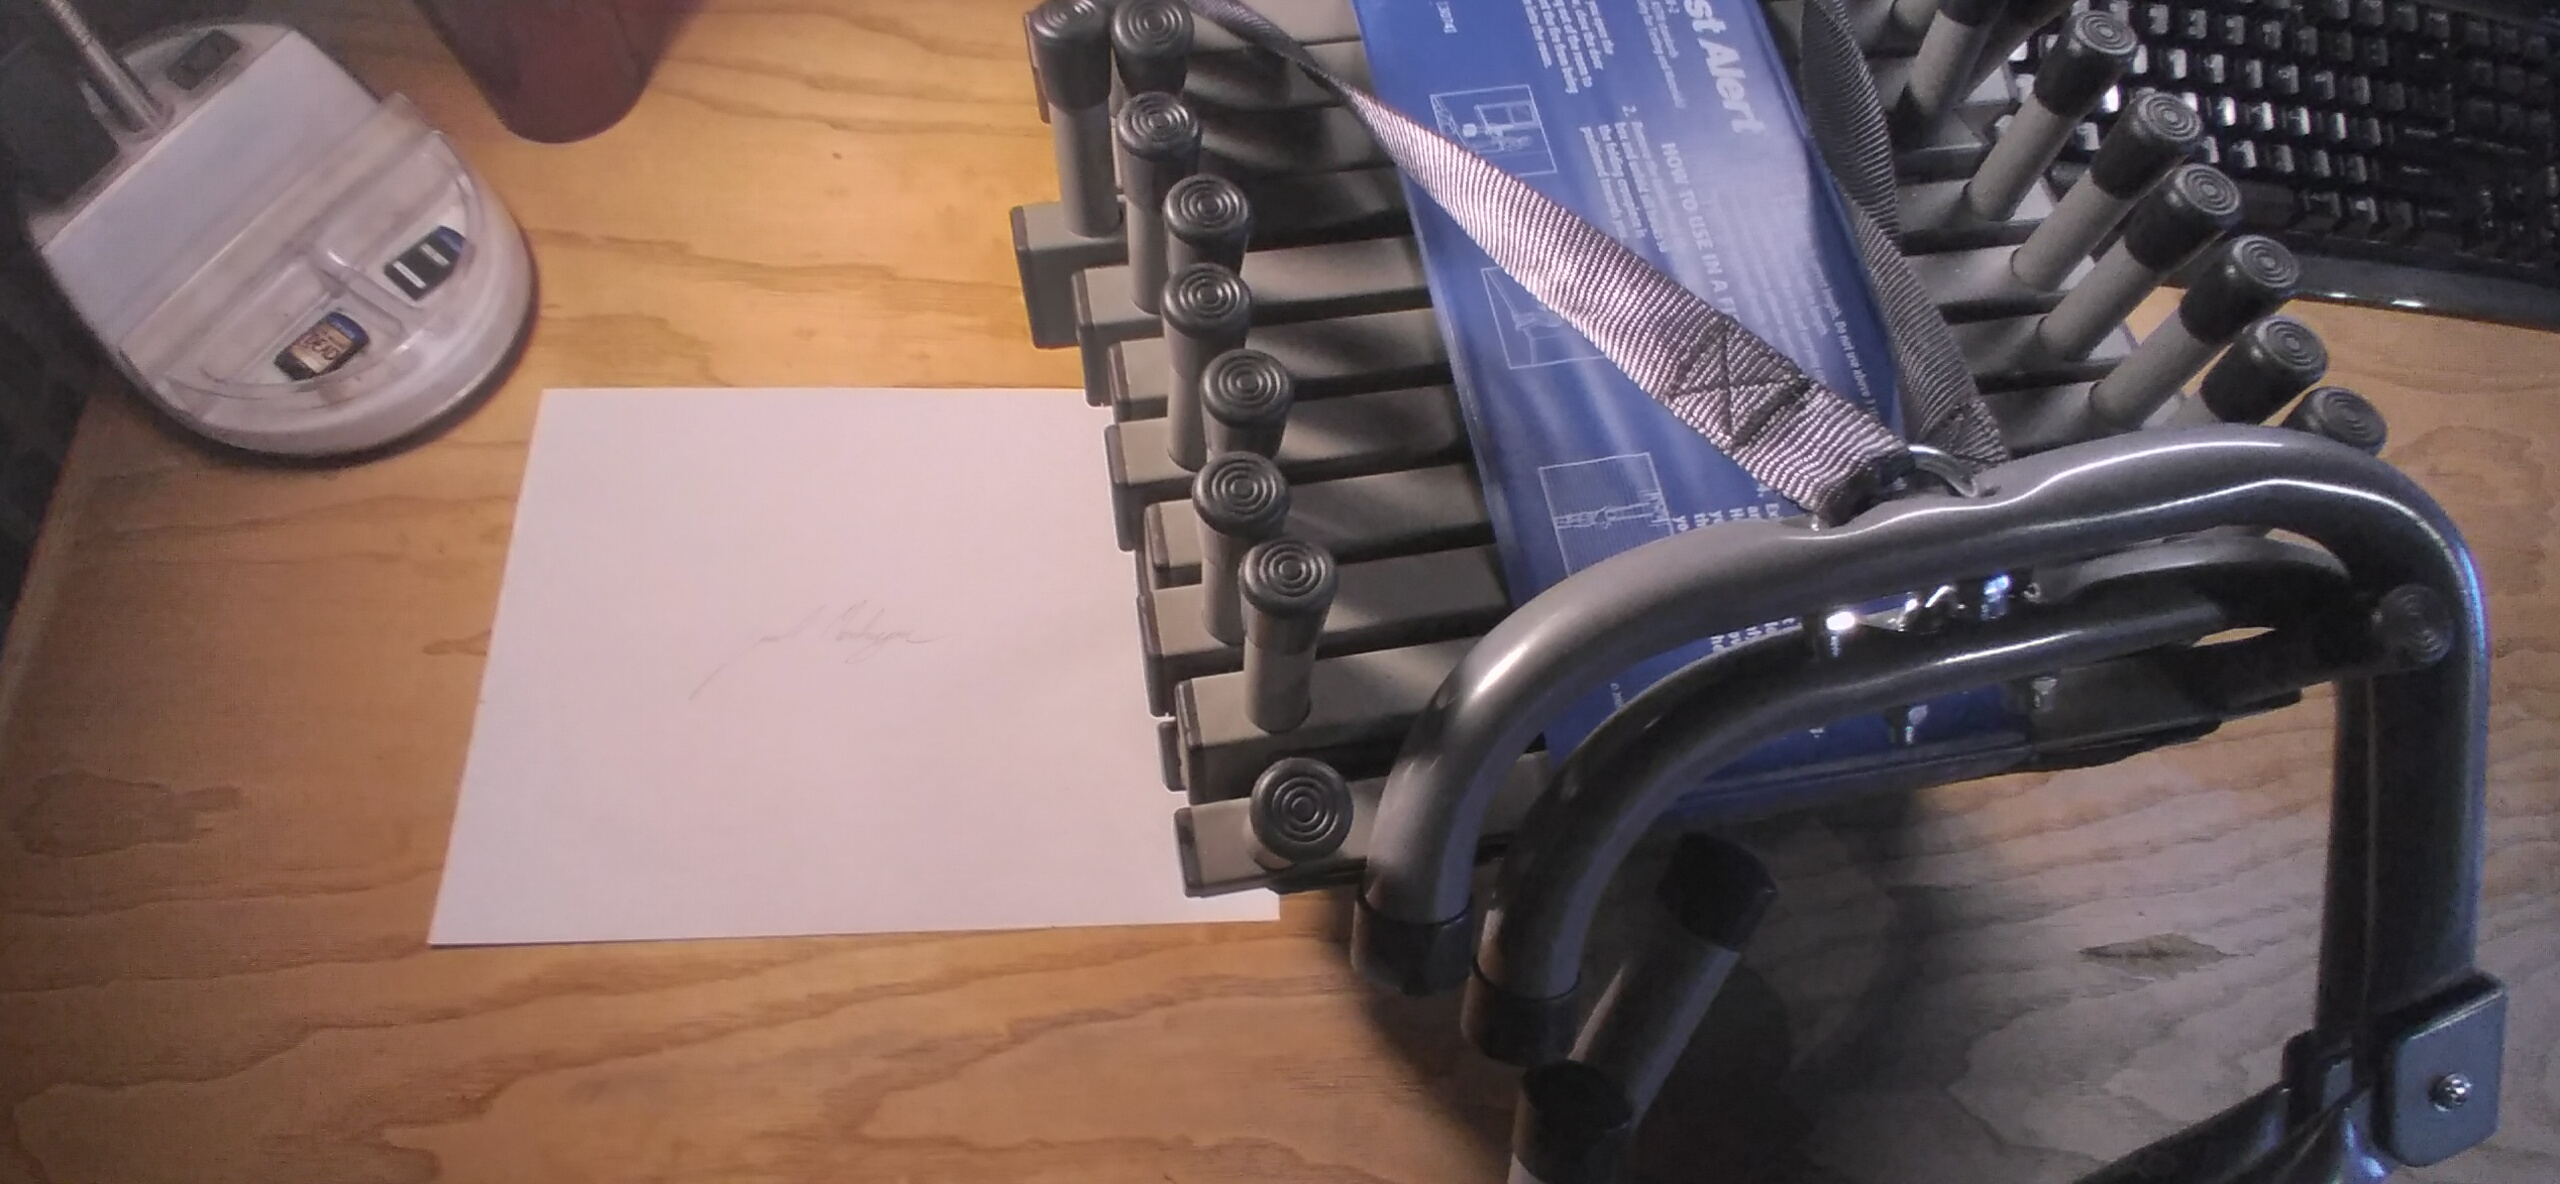
\includegraphics[max width=\textwidth - 6ex]{pics/rope_ladder.jpg}
        \end{center}
        \paragraph~
        \lipsum[1]
    \item{Dagger:}
        \begin{center}
            %\includegraphics[max width=\textwidth - 6ex]{pics/dagger.jpg}
            \includegraphics[max width=\textwidth - 6ex]{pics/necklace.jpg}
        \end{center}
        \paragraph~
        \lipsum[1]
    \item{Vial of Poison:}
        \begin{center}
            \includegraphics[max width=\textwidth - 6ex]{pics/vial_of_poison.jpg}
        \end{center}
        \paragraph~
        \lipsum[1]
    \item{Herbs and Flowers:}
        \begin{center}
            \includegraphics[max width=\textwidth - 6ex]{pics/herbs_and_flowers.jpg}
        \end{center}
        \paragraph~
        \lipsum[1]
    \item{Juliet's Ring:}
        \begin{center}
            %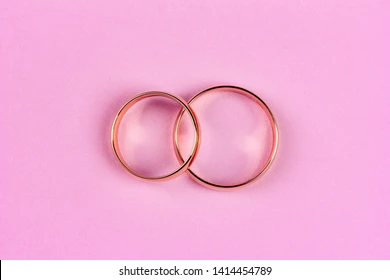
\includegraphics[max width=\textwidth - 6ex]{pics/ring.jpg}
            \includegraphics[max width=\textwidth - 6ex]{pics/necklace.jpg}
        \end{center}
        \paragraph~
        \lipsum[1]
    \item{Juliet's Necklace:}
        \begin{center}
            \includegraphics[max width=\textwidth - 6ex]{pics/necklace.jpg}
        \end{center}
        \paragraph~
        \lipsum[1]
    \item{{\color{blue}\underline{\href{https://www.youtube.com/watch?v=73lj5qJbrms}{All Together Now}}}:}
\end{enumerate}

\section{Original Movie Poster}

\end{document}
